\documentclass[11pt,a4paper,oneside]{article}

\usepackage{pslatex,palatino,avant,graphicx,color}
\usepackage[margin=2cm]{geometry}
\usepackage{hyperref}

\begin{document}

\section{Developers Guide}
This introductury developers guide, aims to make a developer able to set up Stedr so that the developer gets an overview of how the system works and also how the developer can get started programming. The first part of the guide is about the backend while the second part is about the frontend. Both of the guides needs to be completed to get the example program running, and the backend part has to be completed before the frontend part. 

\noindent

This guide is \textbf{not} meant as a tool guide, so some parts of the guide is superficial and it is left to the reader to study the tools closer.

\subsection{Backend}

The backend is a Java program using the Play Framework, and the backend is deployed to the Heroku, a cloud platform hosting applications as services. The source code itself maintained on a GitHub account provided by Sintef called TagCloud. Before continuing this means that a couple of prerequisites has to be fulfilled by the developer.

\paragraph{The developer should have:}
\begin{itemize}
\item Installed an updated version of JDK 
\item Installed a code editor (Eclipse will be used in the tutorial)
\item A working GitHub-account
\item Installed git
\item Cloned TagCloud/StedR\textunderscore server with the help of Git from GitHub
\item Installed the Typesafe Framework from \href{http://www.playframework.com/download}{Play Framework}
\item An \href{https://www.heroku.com/}{Heroku} account 
\end{itemize}  

On your computer, open up a terminal of your choice (cmd, bash, \dots) and navigate to the folder where you have extracted Typesafe Activator (Play Framework). Depending on your platform type the command which will executeactivator. It is possible to use Typesafe Activator with a graphical user interface by passing ui as a parameter. This will look something like:
\begin{center}
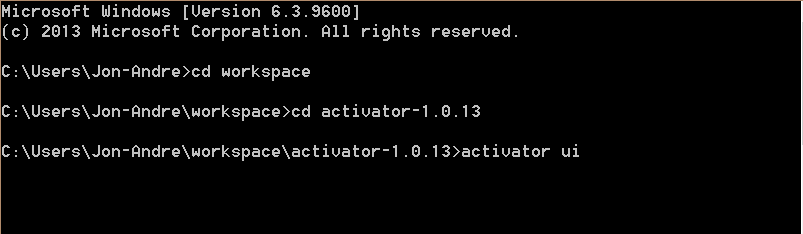
\includegraphics[scale=0.8]{guide/activator1.png} 
\end{center}
The graphical user interface should then open automatically in a browser view. If this doesn't happen check the terminal for error messages.

\paragraph{}
In the right sidebar navigate to the folder where you have cloned StedR\_server from GitHub. Click choose. Now the program is starting to compile, and the server will try to run as a local instance on \href{http://127.0.0.1:9000}{localhost port 9000}. 
\begin{center}
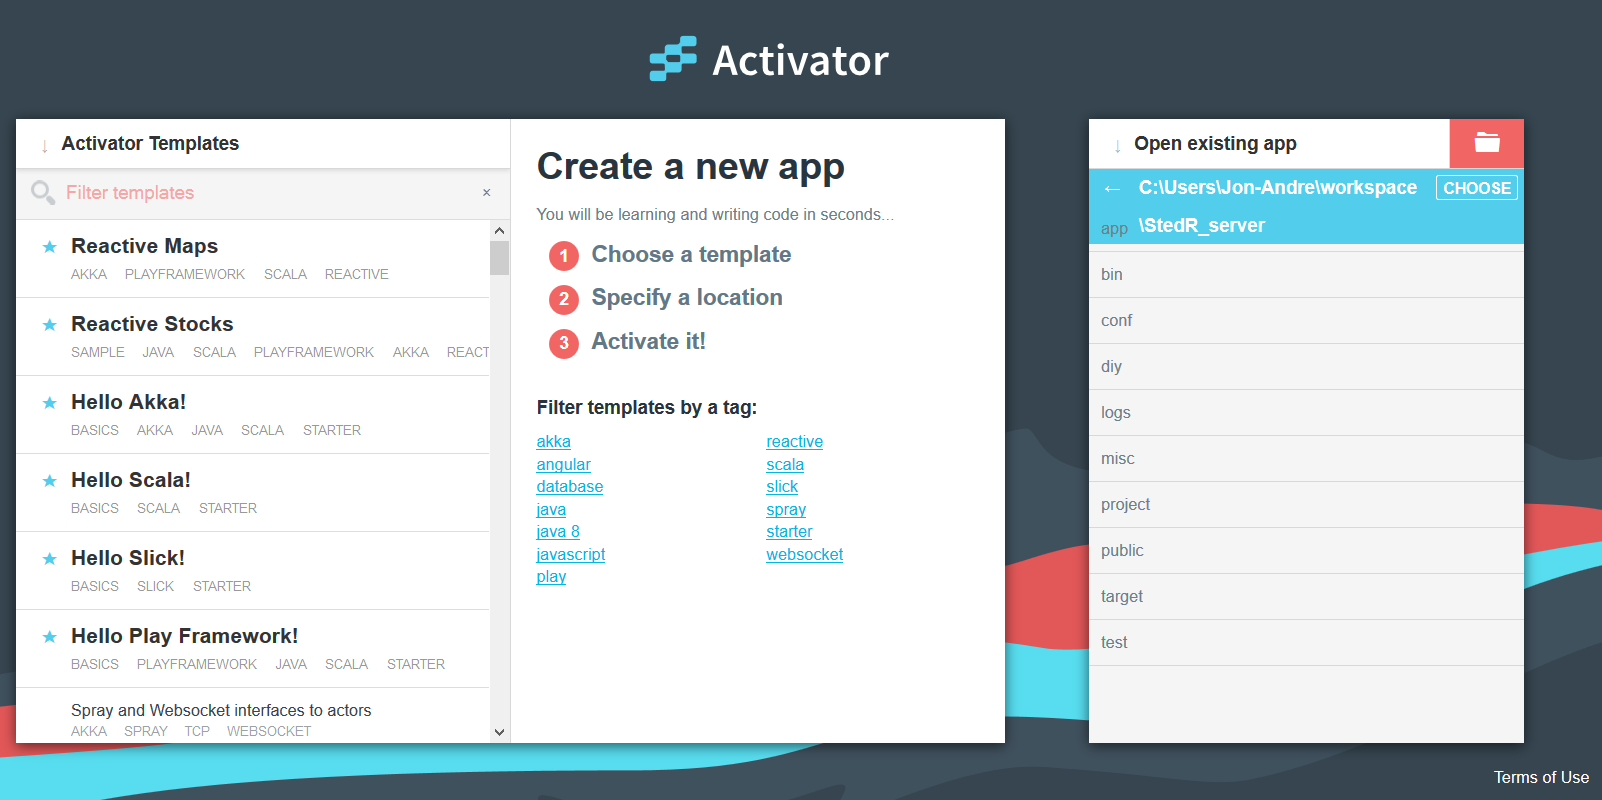
\includegraphics[scale=0.4]{guide/activator2.png} 
\end{center}

Notice that Typesafe Activator itself is running on port 8888. During the compiling of the system problems may occur. Often this is related to a mismatch between Typesafe and Java, for example an updated version of Java and an unupdated version of Typesafe often leads to issues. If the program is compiled succesfully, something like this should appear at localhost: 

\begin{center}
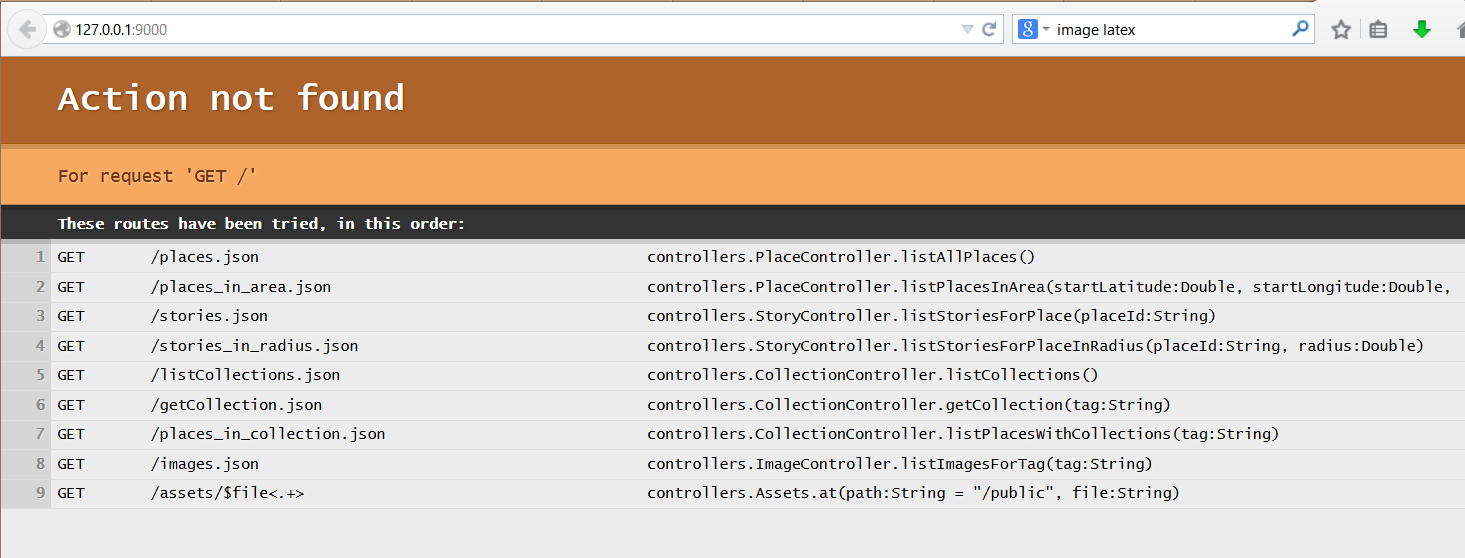
\includegraphics[scale=0.5]{guide/activator3.png} 
\end{center}

If you already have tried importing the folder with the source code to an editor like Eclipse, you may have noticed a lot of errors appears. To import the program and its dependencies as a project: In the left sidebar of Typesafe, click on Code, then the gear-icon. Here you can choose between Intellij and Eclipse, and Typesafe will then generate project files and guide you through how to open the program as a project. 
\begin{center}
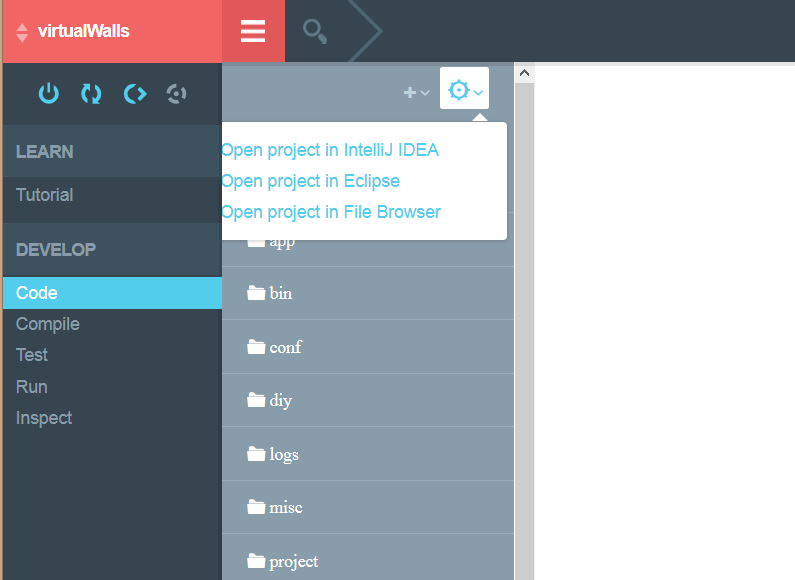
\includegraphics[scale=0.6]{guide/activator4.png} 
\end{center}
Now you should have a running instance of the server locally, and you're also ready to code. 

\paragraph{}

In Eclipse you will get an overview of the different source files and source packages. In the \texttt{Controllers} package you will find \texttt{controllers} that take care of identifying queries (sent as an URL), creating \texttt{Retrievers} that process the queries and at last returning a response to the query. All of the  \texttt{Controllers} are written by former Stedr-developers, but all of the  \texttt{Controllers} extends a  \texttt{Controller} from the Play Framework.

\begin{center}
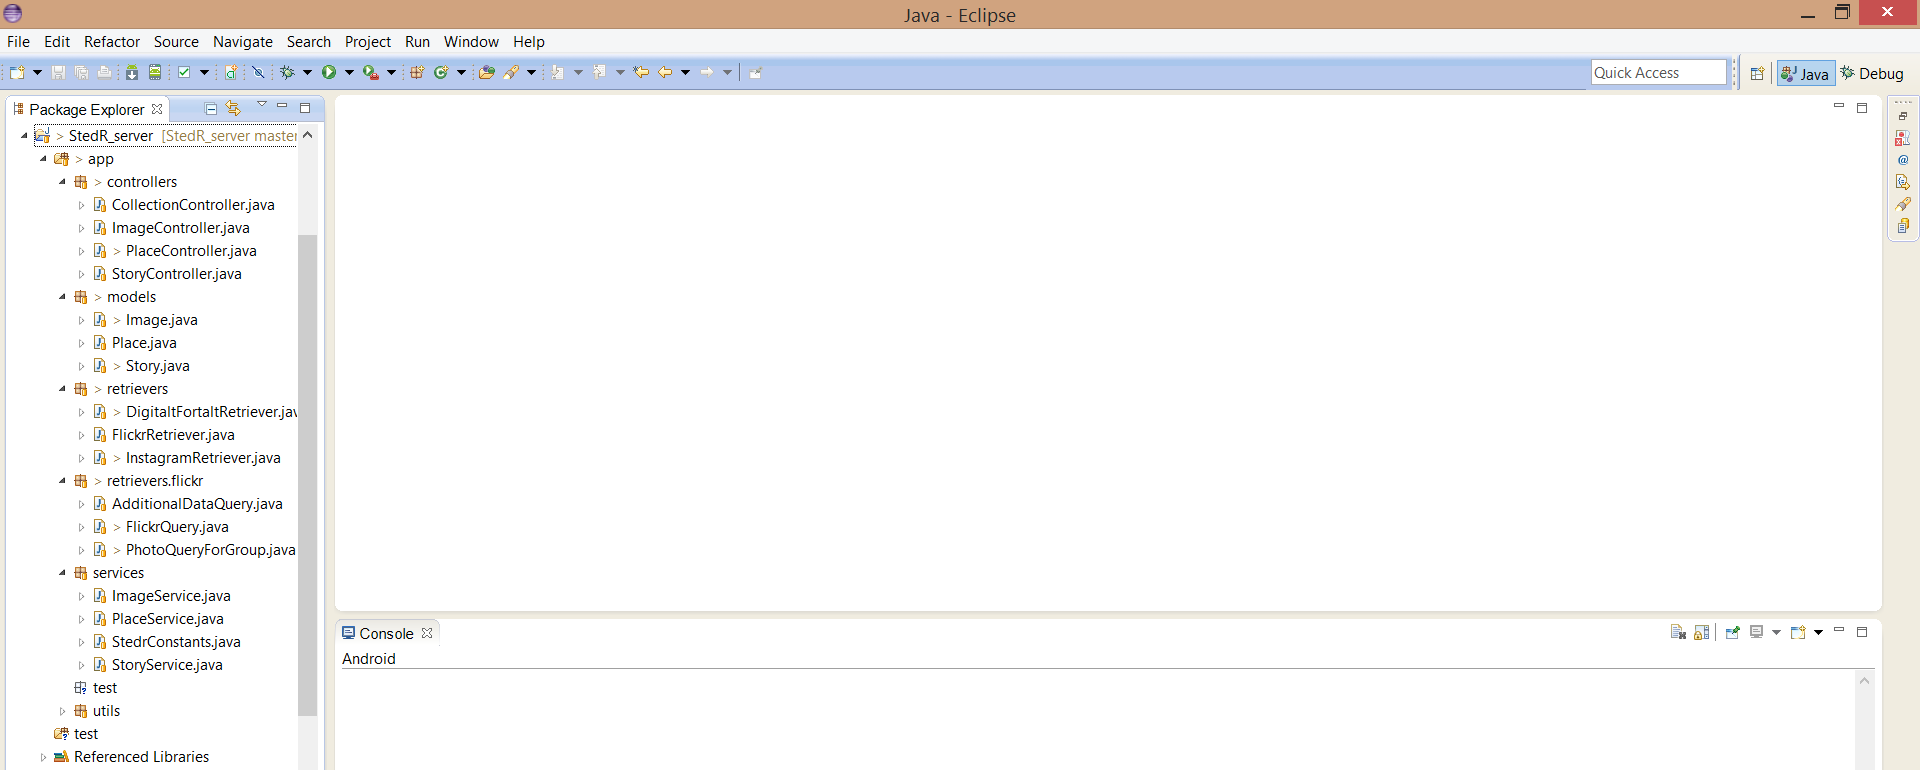
\includegraphics[scale=0.4]{guide/eclipse1.png} 
\end{center}

Now, let's create a controller for our example application:


\begin{center}
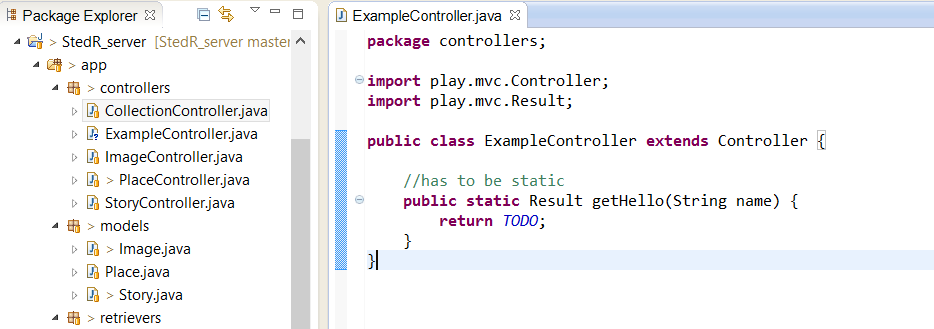
\includegraphics[scale=0.7]{guide/eclipse2.png} 
\end{center}

We ask for a parameter called \texttt{name} which naturally is the name you want to be displayed in the smartphone-application. To pass a parameter you have to edit the file called \texttt{routes} in the conf-folder, the passing is done directly from the smartphone application.

\begin{center}
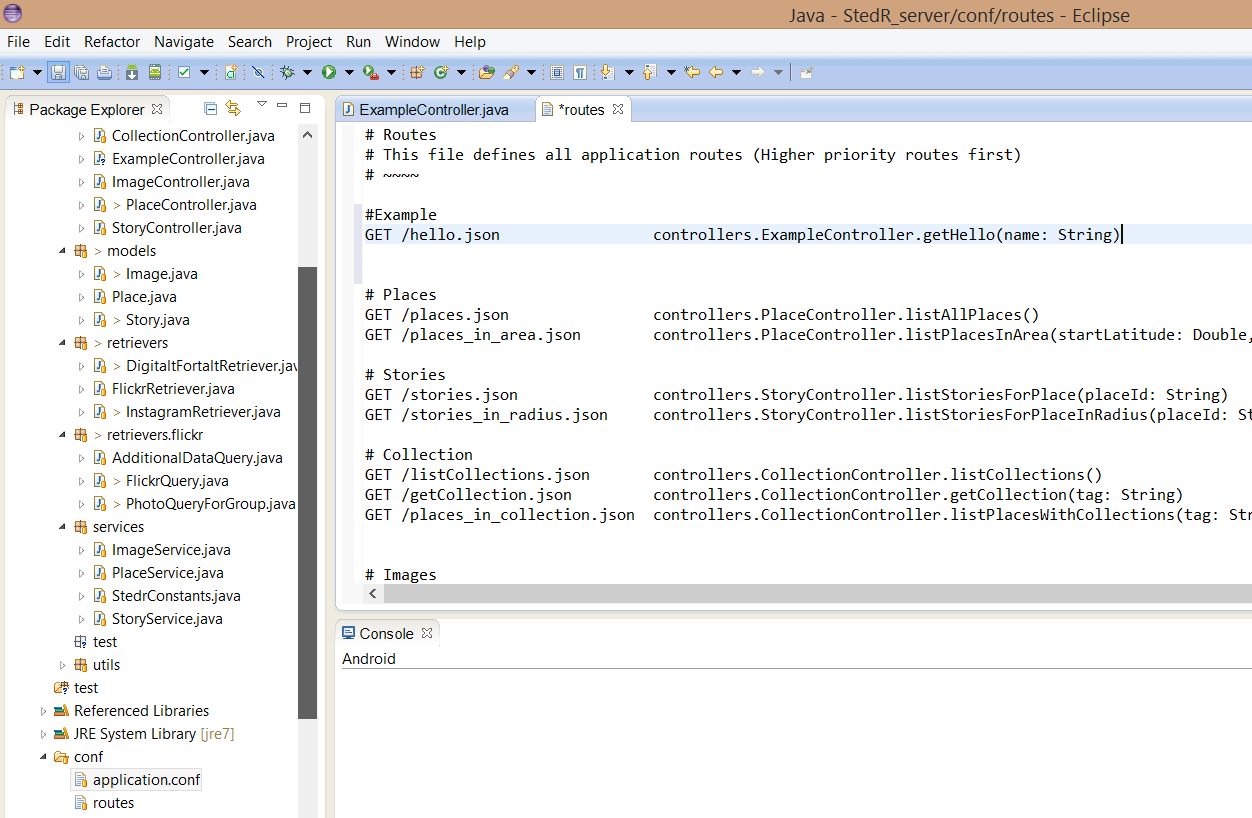
\includegraphics[scale=0.5]{guide/eclipse3.png} 
\end{center}

It would now have been possible to create a \texttt{retriever} directly, but we won't do that. In the services folder there are three files ending with  \texttt{Service.java}. These files are interfaces, and the reasoning behind them is that it should be easy to add or change services. As of now stories are provided by Digitalt Fortalt, so we have a \texttt{DigitaltFortaltRetriever.java} which implements \texttt{StoryService.java} That way we can change the content provider to Wikipedia by creating a new retriever \texttt{WikipediaRetriever.java} which implements \texttt{StoryRetriever.java} A lot of code would then have to be written in order to get the fictional \texttt{WikipediaRetrever.java} functional. Back to the example we will therefore create an ExampleService. 

\begin{center}
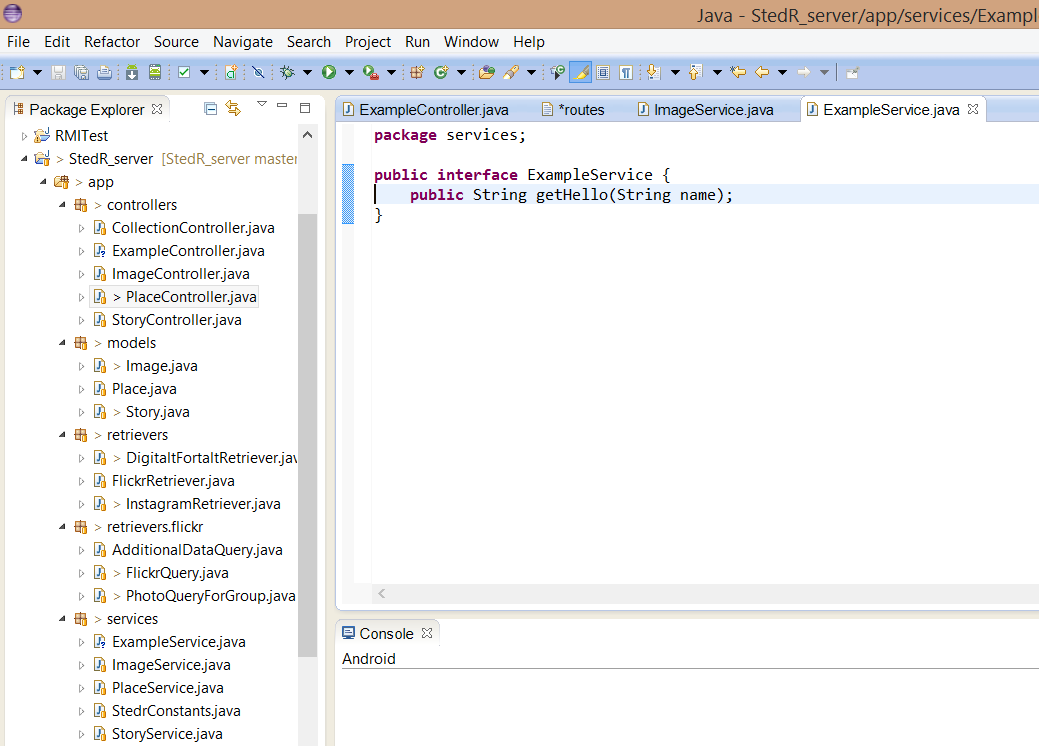
\includegraphics[scale=0.7]{guide/eclipse4.png} 
\end{center}

Now we're ready to implement the \texttt{HelloRetriever}

\begin{center}
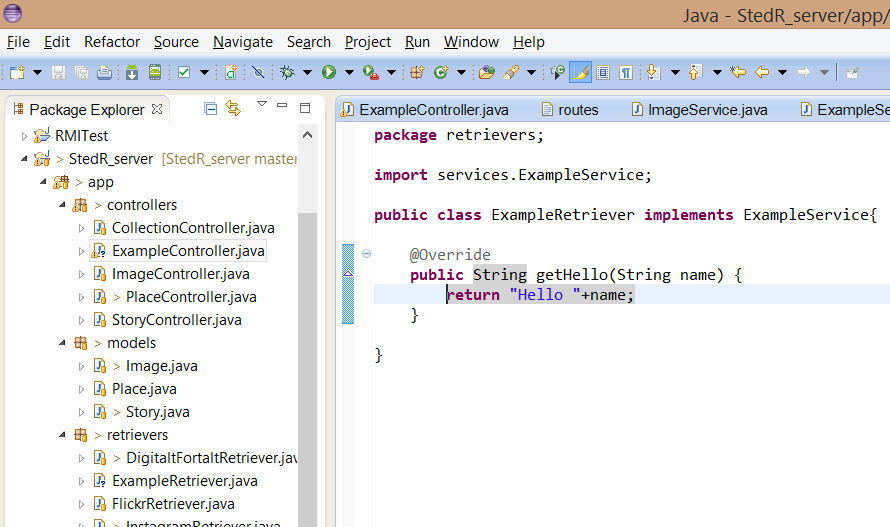
\includegraphics[scale=0.7]{guide/eclipse5.png} 
\end{center}

After the \texttt{HelloRetriever.java} the last thing that needs to be completed is the ExampleController which was created in the beginning of the example

\begin{center}
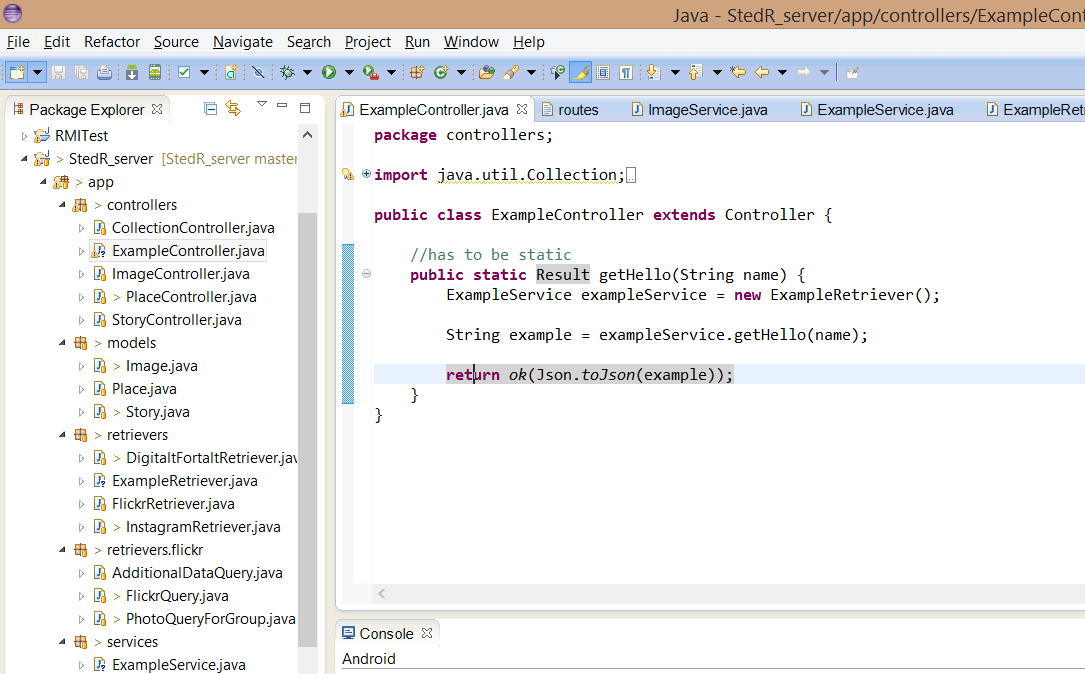
\includegraphics[scale=0.6]{guide/eclipse6.png} 
\end{center}

This concludes in a server which will respond with \texttt{Hello World} if  \texttt{World} is passed as a parameter. To see this, the system has to be recompiled in TypeSafe Activator. After recompiling open \href{http://127.0.0.1:9000}{localhost port 9000}, there you should see:

\begin{center}
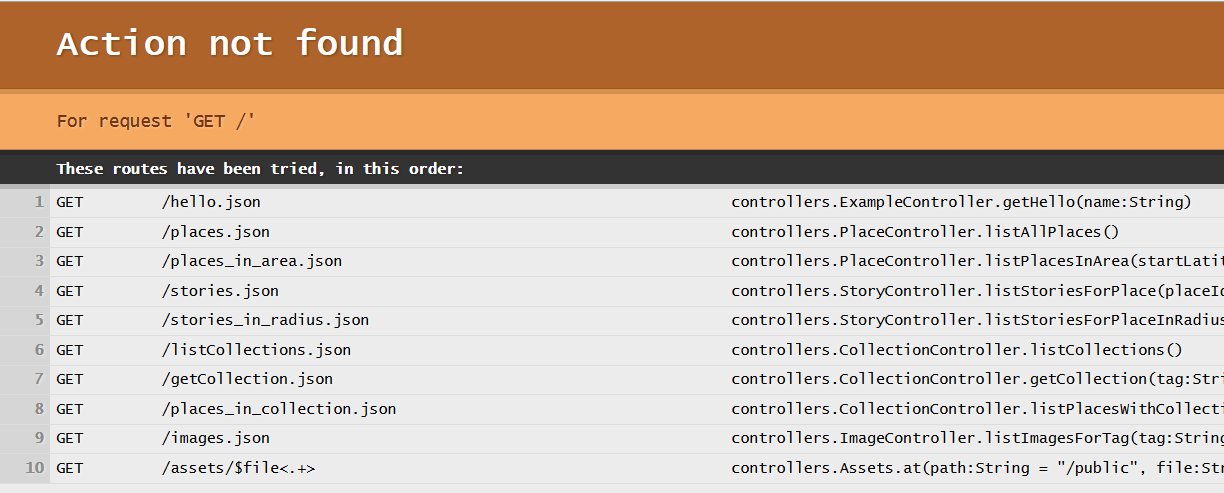
\includegraphics[scale=0.6]{guide/localhost.png} 
\end{center}

If this is correct,  \href{http://127.0.0.1:9000/hello.json?name=world}{http://127.0.0.1:9000/hello.json?name=world} should give:

\begin{center}
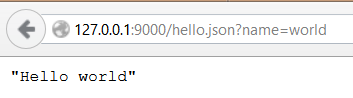
\includegraphics[scale=0.8]{guide/completed.png} 
\end{center}

Normally you would commit this to the git-repository on GitHub, and if the new functionality is to be a part of the running server it should also be commited or deployed to Heroku. This is done by pushing the server to \texttt{git@heroku.com:stedr-beta.git}. Note that in order to push to the server directly, you will need contributor access to stedr-beta.herokuapp.com. If this isn't available or provided upon request you can create a new Heroku instance, but then the request URL destinations have to be changed in the smartphone application.

\section{Frontend}

\dots

\end{document}
